% Chapter 1

\chapter{Introduction} % Main chapter title

\label{introductionchapter} % For referencing the chapter elsewhere, use \ref{Chapter1} 

%\lhead{Chapter 1. \emph{Introduction}} % This is for the header on each page - perhaps a shortened title
\lhead{Chapter \ref{introductionchapter}. \emph{Introduction}} % This is for the header on each page - perhaps a shortened title

%----------------------------------------------------------------------------------------
\section{Background}
Obesity and overweight are currently global health concerns. In one systematic review, it was revealed that overweight and obesity had a tendency to be linked to an increase of incidence of several co-morbidities, for example, type 2 diabetes and other chronic conditions like cardiovascular diseases and cancer~\citep{guh2009incidence}. The number of people who are considered to be either overweight or obese stands at approximately 1.3 billion~\citep{steyn2006chronic}. A survey by~\cite{abegunde:theburden}, which included a total of 23 low-income and middle-income countries, projected a loss of US\$84 billion in economic production between 2006 and 2015 from heart disease, stroke and diabetes alone, in the absence of any significant measures put in place to intervene.

Co-morbidities that are associated with obesity are likely to inundate healthcare systems~\citep{pollak2010s}. Todate, healthcare systems have failed to optimally treat chronic conditions such as diabetes due to the lack of time for providing continuous patient care, which is essential in the management of chronic conditions~\citep{quinn2008welldoc}. Resources are insufficient to deal with an overwhelming increase in number of patients, hence there have been suggestions to move part of the care to the hands of patients~\citep{aarsand2012mobile}.~This need calls for innovative and citizen-centric  interventions to foster lifestyle changes, in order to both prevent or delay the onset of chronic conditions in populations, and support patients in self-management of chronic conditions, to reduce the burden on healthcare systems~\citep{korhonen2010personal,aarsand2012mobile,higgins2016smartphone}. There has been a growing number of initiatives by both commercial and research communities to develop mobile applications and wearable sensors that could nudge individuals to eat healthily and increase their level of physical activity~\citep{chen2014healthytogether}. Citizen-centric interventions are now possible due to advancements in hardware and software technologies, which have facilitated the creation of opportunities for automation of health self-management processes~\citep{arsand:mobile}. 

One interesting trend in both academia and industry is the use of mobile phones in health. The mobiles have become an effective means of ``just in time'' delivery of interventions that target psychological processes~\citep{hsu2014persuasive}. These devices are currently omnipresent and people carry them most of the time~\citep{mattila2008mobile}, hence their presence adds a ``kairos factor'' to the delivery of interventions that target both health promotion~\citep{pollak2010s} and persuasion~\citep{hsu2014persuasive}. Smartphone-based applications have been rapidly gaining popularity as effective tools to support delivery of personalized health information~\citep{handel2011mhealth}. One of the prevalent uses of mobile health apps is self-monitoring, to augment \emph{cognitive behaviour therapy} -- the treatment of behaviour in clinical settings~\citep{mattila2008mobile,medynskiy2010salud}. These apps facilitate the data collection of one's health parameters through inbuilt tools such as GPS and an accelerometer (body activity sensor); hence they present an innovative way of monitoring and improving both health and fitness~\citep{higgins2016smartphone}. In order for such tools to support changes in health behaviour and the promotion of a healthy lifestyle, theory-based strategies such as gamification (for enhancement of motivation), enabling self-reflection through goal setting and feedback (for improvement of self-efficacy), and SMS reminders are often applied~\citep{consolvo2009goal,cole2010text,hamari2014persuasive,hamari2014does,higgins2016smartphone}. However, such tools have limitations when they are used in specific contexts. The basis of the research problem for this study was to address the limitations inherent in the developing world context but these limitations can as well scale to a context of developed world. The research problem is as reported below.
\section{Statement of the Problem}
A review by~\cite{higgins2016smartphone} presented evidence that self-monitoring apps can help patients reach their health and fitness goals.~These apps can also support individuals who are not patients to become aware of their behaviours, which is an important step towards taking actions that are necessary to live a healthy lifestyle. However, such apps have limitations as they don't accommodate specific interaction modes that involve the sharing of devices and indirect usage. Such modes of interaction are prevalent and relevant in the context of the developing world, and self-monitoring applications that are designed for direct use may not replicate well in some populations of users~\citep{kaplan2006can,sambasivan2010}, especially when users face barriers to direct access of user interfaces or technology~\citep{kumar2015mobile}. Typically, self-monitoring apps utilize  specific theory-informed motivational affordances in order to enhance the engagement of end users. But such incentives have been designed only for a direct user and are not supported in a situation where there are at least two layers of users that consist of an intermediary user, who acts as a bridge for an indirect user, and the indirect (beneficiary) user of information in a self-monitoring app. Such a scenario of intermediated technology is shown in Figure \ref{figure:directVSinterm}, which is profoundly explained by~\cite{sambasivan2010} from the perspective of activity theory~\citep{kaptelinin1997activity}. In a direct interaction, a computing device or system is an object that provides specific affordances of activities that an end user can perform on the object, while in an intermediated interaction there is an additional layer of human interface: the intermediary user, responsible for translating the intents of a beneficiary user into actions, by carrying out activities on a computing device or system on behalf of an indirect user (the beneficiary user).
\begin{figure}[htbp]
  \centering
    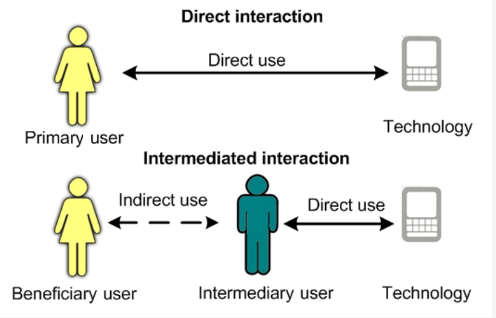
\includegraphics[width=0.6\textwidth]{Figures/intermediated.png}
    \rule{35em}{0.5pt}
  \caption{Direct and intermediated interactions~\citep{sambasivan2010}.}
  \label{figure:directVSinterm}
\end{figure}

This research explored how one could support personal health informatics technology where its usage is facilitated by intermediary users on behalf of beneficiary users (indirect users). Despite a vast amount of literature on \emph{intermediated technology use}, such persuasive technologies have not been extensively explored in this context. Persuasive technologies tend to have their unique design considerations, and intermediated technology use has its socio-technical aspects; hence one has to understand which factors to consider and how to go about implementing a useful intervention that could work in such a complex context. This study had two main research questions, as presented below.
\begin{enumerate}
%\setcounter{enumi}{1}
\item What is the role of social-technical settings in the intermediated use of gamified self-monitoring applications targeting the promotion of healthy eating and physical activity?

\textbf{Sub-questions}
\begin{enumerate}[label=\alph*.]
\item What social factors have impact on the intermediated use of a gamified self-monitoring application?
\item To what extent do those social factors affect motivation to engage with a gamified self-monitoring application in intermediated use context?
\end{enumerate}
\item How does gamification play a role in motivating the intermediated use of self-monitoring applications targeting the promotion of healthy eating and physical activity?

\textbf{Sub-questions}
\begin{enumerate}[label=\alph*.]
\item What is the impact of gamification on supporting the self-determination of intermediary users to engage with a self-monitoring application in intermediated use?
\item What is the impact of gamification on supporting the self-determination of beneficiary users to engage with a self-monitoring application in intermediated use?
\item What is the impact of gamification on the frequency of utilizing the self-monitoring application in intermediated use?
\item What is the impact of gamification on the motivation of beneficiaries to self-monitor diet?
\item What is the impact of gamification on the motivation of beneficiaries to self-monitor physical activity?
\item How does the presence of gamification affect the relationship between the two members of a pair participating in intermediated use?
\item To what extent might gamification encourage or discourage internalization of intermediated use behaviour?
\end{enumerate}
\end{enumerate}  
\section{Research Contribution}
This research grounded its findings from user evaluations, ideas from past studies and  existing theories of human motivation.~User evaluations included a total of three studies, carried out in three townships in South Africa at non-overlapping intervals of time. Each user study helped to uncover unique insights that were important in getting answers to the aforementioned research questions. Each user study consisted of several pairs of users.~Each pair of users consisted of one beneficiary user (a person who solicited help in using the self-monitoring application), and one intermediary user (a person who provided the required help to a beneficiary user: to facilitate interaction with the self-monitoring application). Beneficiary users elected their respective intermediary users and the pair had access to the app for a certain number of days before questionnaires and interviews were administered.  

Data collection techniques consisted mostly of the triangulation of the app's usage logs, interviews and questionnaires. In order to solve the problem, prior to carrying out any prototype development and evaluation, the study started with a contextual investigation to gain a preliminary understanding of users' context. The process involved administering semi-structured questionnaires to adult participants whom the research team opportunistically approached in a hospital setting in Cape Town. Iterations of software development and informative evaluations of mobile application prototypes, followed after the contextual investigation. Motivational affordances implemented on prototypes included gamification features such as leaderboards, badges, avatars, virtual pets and social interaction features.  Through the course of eliciting feedback from user studies, I as the researcher was able to generate insights in an iterative manner, where each iterative user study informed the formulation and execution of a successive user study. 

From informative evaluations, the study concluded with a summative evaluation which aimed to measure the effectiveness of using gamification in the promotion of intermediated use of self-monitoring applications. 
 
The contribution of this research is mainly to increase understanding of which social dynamics and motivational affordances to consider when designing personal health informatics (PHI) for intermediated use. In this dissertation it is suggested that rather than designing PHI for the beneficiary alone, one can design for intermediated use, explicitly acknowledging the presence of intermediary users as facilitators of access to a self-monitoring application.~This research demonstrated that it is feasible to frame the design of personal applications in a way that promotes collaboration between an intermediary user and a beneficiary user, hence reaching the goal of motivating intermediated use. The dissertation highlights some social configurations that are crucial for the intermediated use of a self-monitoring application. The dissertation further emphasizes the importance of pairing users within family settings to foster an environment that encourages intermediated use.  The study indicated that when a pair consists of immediate family members, the prior social relationship may promote internalization of help-giving behaviours on the part of intermediaries. Prior social relationship appears to be a prerequisite for setting up an intervention, and it can provide rationale for intermediaries to perceive gamification as something that is fun to use but, at the same time, as something done to support a good cause, which in this case was to help someone they care about. With the presence of that care, and by adding a gamification layer,  collaboration and family bonds show indications of improvement.~However, in some situations competition appears to harm an existing family bond between members of a pair instead of promoting it, especially when one member of a pair feels let down by the other member of the pair.~Strengths and weaknesses of different motivational affordances in terms of promoting aspects of autonomy, competence and relatedness are also discussed in detail, in order to offer insights to both designers and researchers for the design of future interventions.
\section{Thesis Organization}
I have organized this thesis as follows. Chapter 1, \emph{\textbf{Introduction}}, provides the background information of the problem, research questions, and the contribution of this research to knowledge. Chapter 2, \emph{\textbf{Literature Review}}, mainly covers  the theoretical underpinning of this research in terms of related work and the conceptual framework that lays a foundation for this research. Chapter 3 is on \emph{\textbf{Study Context}}, which situates this work in the South African context by providing a rationale for carrying out a study in South African townships. Chapter 4 presents the \emph{\textbf{Contextual Enquiry}}, which we conducted at the beginning of the study to understand how technology is being utilized in general in the context of older adults who are prospective beneficiary users of the technology. In addition, this contextual enquiry aimed to uncover whether there were particular usages of technology that were health related. Chapter 5, \emph{\textbf{Prototype I}}, describes the development and evaluation of the first prototype. In the development part, I generated the preliminary user requirements after combining insights gained from both the preliminary findings of the contextual enquiry and ideas grounded in literature. Chapter 6, \emph{\textbf{Prototype II}}, covers the improvement of the first prototype. The research used both qualitative feedback from the evaluation of the previous prototype, and his direct observation of context in the field, to guide the improvement. Chapter 7, \emph{\textbf{Summative Evaluation}}, is where I evaluated the second prototype with a placebo group to discern the isolated effect of gamification on existing family bonds. Chapter 8, \emph{\textbf{Conclusions and Future Work}}, discusses how the whole study addressed the research questions and highlights reflection on the three evaluation studies, by providing insights on design lessons learned from the strengths and weaknesses of the gamified personalized application for intermediated use. In addition, this last chapter includes takeaways from this research and introduces the basis for future research.         
\begin{flushright}
\end{flushright}
